\chapter{Introduction}\label{ch:intro}

Human cognition relies on the ability to sense, process, and understand the surrounding environment and its sounds.
Although the skill of listening and understanding their origin is so natural for living beings, it still results in a very challenging task for computers. In recent years several novel methods have been proposed to analyze this information automatically, and several new applications have emerged \cite{virtanen2018computational}. However, the creation of ``machine listening'' algorithms that can mimic this cognitive feature by means of artificial systems remains a very challenging task. 

Automatic sound event detection (SED), also known as acoustic event detection, is nowadays considered as one of the most important topics in the field of computational auditory scene analysis (CASA). Thanks to works like Bregman's ``Auditory Scene Analysis: The Perceptual Organization of Sound''~\cite{bregman1994auditory}, we can trace back the birth of this field to 1994, when the field of auditory scene analysis (ASA) was introduced in order to model humans' sound perception. Following this work, many other contributions were written aiming to describe how artificial systems can be designed in order to perceive sounds similarly to as humans do; most of these works will be later collected in Divenyi's book~\cite{divenyi2004speech} in 2004. Labels extracted with a SED system usually allow us to achieve a better insight of the considered acoustic scenario, for example they can be used as mid-level representation useful for other CASA research areas. In~\cite{chu2009environmental, heittola2010audio}, for example, authors make use of SED for designing audio context recognition systems, while in~\cite{shah2012lifelogging} and~\cite{wichern2010segmentation} SED is exploited for automatic tagging and audio segmentation respectively. Moreover, SED also found many direct applications in a variety of scenarios, some examples being context-based indexing and retrieval in multimedia databases~\cite{xu2008audio}, unobtrusive health monitoring~\cite{peng2009healthcare}, and audio-based surveillance~\cite{harma2005automatic, crocco2014surveillance, Principi2016a}.

In the recent years, the research on automatic-assisted home environments has been an active area for study, with particular attention to the processing of audio signals \cite{Gemmeke13,Vacher2015,Principi2015a}. Typically, to increase the quality of the audio signal and improve the performance of the successive audio analysis stages in complex systems, pre-processing algorithms are employed \cite{loizou2013speech,Hussain2007,Rotili12b}. In addition, nowadays one of the main subject of interest in technological research regards systems deployed for surveillance applications. Surveillance can be seen as control of public safety or as the supervision of private environments where people may live alone.  The increasing level of public security over the past decades has motivated the installation of sensors such as cameras or microphones in public places (stores, subway, airports, etc.), while is possible to effectively consider personal multimedia devices (smartphones, tablets, etc.) as virtual assistant which is able to monitor the user and eventually intervene in case of necessity without having the need for a physical interface (i.e., keyboard) anymore.
Thus, the need of unsupervised situation assessment stimulated the signal processing community towards experimenting with several automated frameworks, due to their potential in several engineering applications.
In these contexts, sound or sound sensing can be advantageous with respect to other modalities of multimedia processing, due to the short duration of certain events (i.e., a human fall, a gunshot or a glass breaking) or the personal privacy motivate the exploitation of the audio information rather than, e.g., the image processing. 
In addition, audio processing is often less computationally demanding compared to other multimedia domains, thus embedded devices can be easily equipped with microphones and sufficient computational capacity to locally process the signal captured. 
These could be smart home devices for home automation purposes or sensors for wildlife and biodiversity monitoring (i.e., bird calls detection \cite{grill2017two}). 
Some of these applications have already become commercial products that are able recognize certain specific sound categories in realistic environments and improve home security \cite{audioanalytic}  or companies with as much impactful missions, such as preserve the Rainforest from illegal deforestation \cite{rainforest}.

The type of information to be extracted with these algorithms depends on the application. In particular, we can sort the sound analysis tasks explored in this work into two high-level categories: sound event \textit{detection} and sound event \textit{classification}.
In sound event detection, or acoustic event detection, the goal is to detect the onset and offset times for a variety of sound events captured in an audio recording. 

In sound event classification, the goal is to categorize an audio recording into one of a set of predefined categories by associating a textual descriptor.

In controlled laboratory conditions where the data used to develop computational sound scene and event analysis methods matches well with the test data, it is possible to achieve relatively high accuracies in the detection and classification of sounds.  However, there are several complexities in computational sound analysis and current technologies face many challenges, mainly related to the acoustics of sound scenes and events, when they are employed in realistic environments.
Among these challenges we can include:
\begin{itemize}
	\item the effect of the environment acoustics: reverberation, background noises and the channel coupling (impulse response) between the source and the recording equipment;
	\item the intra-class variability, i.e., high difference of the acoustic characteristics of even a single class of sounds and on the other hand the similarity of many different types of sounds to the target events  \cite{stowell2015acoustic};
	\item the \textit{polyphony}, i.e. the occurrence of multiple simultaneous events. In realistic environments there
are almost always multiple sources producing sound at the same time. 
\end{itemize}

In addition to these complications related to the acoustics of sound scenes and
events, there are also several fundamental limitations related to the computational methods. In particular, to develop effective models based on the \textit{deep learning} paradigm, a very large set of examples of the
target (and non-target) sounds is required. In contrast to the situation in image classification,
 currently available datasets that can be used to train such systems are more limited in size, diversity, and number of event
 instances, even though recent contributions such as AudioSet \cite{gemmeke2017audio} or the DCASE challenges
and related workshops \cite{DCASE2017Workshop, mesaros2016tut, dcase2018web} have provided public available datasets to reduce this gap.



\section{The Deep Learning Approach for Sound Event Detection and Classification}

\begin{figure}[b]
	\centering
	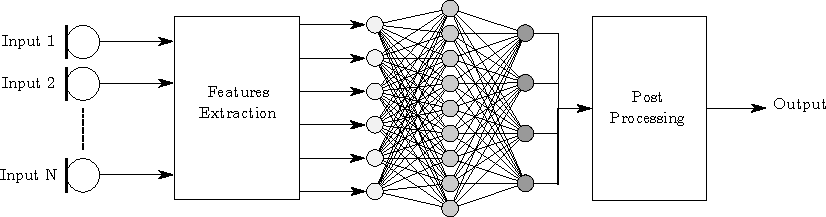
\includegraphics[width=\linewidth]{img/flowchart_1.pdf}
	\caption[Basic structure]{Basic structure of an audio analysis system.}
	\label{fig:base-system}
\end{figure}

\begin{figure}[tb]
	\centering
	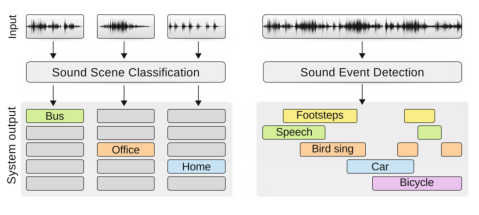
\includegraphics[width=\linewidth]{img/sed_sec.pdf}
	\caption[System input and output ]{System input and output for the two main analysis systems: sound scene classification and sound event detection.}
	\label{fig:system-io}
\end{figure}

The typical computational sound scene
or event analysis system based on machine learning is
depicted in \figref{fig:base-system}, while the different input and output respectively for classification and detection systems
are illustrated in \figref{fig:system-io}.

As the first stage, all the systems take as input one or more audio
signals, either in real-time, captured by a microphone, or offline, from an
audio recording. In this work, we assume always discrete-time signals,
obtained by using analog-to-digital converters. 

The \textit{Feature Extraction} block consists
of different processing stages and outputs acoustic features, as the actual analysis of
audio is rarely based on the raw audio signal, but rather on the compact signal
representation with features. The purpose of the feature extraction is to obtain
information sufficient for detecting or classifying the target sounds, making the
subsequent modeling stage computationally cheaper and also easier to achieve with
limited amount of development material. Very often the feature extraction procedure is also preceded by the down-mixing the audio signal into a single (mono) channel and re-sampling it into fixed sampling frequency.
Although every application could require a specific set of features able to highlight the discriminating particularities of each data sample, the most common representations used
for audio signals are non-linear representation for magnitudes (power spectra and logarithm) and nonlinear frequency scaling (mel-frequency scaling). 
More details of the acoustic features extraction process for each examined case-study will be provided in further chapters.


The \textit{Deep Learning}-based model takes the acoustic features as input and it is trained to produce an output which will assign a class label depending on the application. Almost all the system presented in this work are based on the supervised machine learning approach, where the system is trained using labeled examples of sounds from each of target sound type. 
At the development stage, the obtained acoustic features are used together with
reference annotations of the audio training examples, to learn models for the
sound classes of interest. Annotations contain information about the presence of
target sound classes in the training data, and are used as a reference information
to automatically learn a mapping between acoustic features and class labels. The
mapping is represented by acoustic models. The learning process consists in updating the parameters or \textit{weights} of the neural network, searching for the optimal model that minimize a certain cost-function. 
At the usage stage, the learned acoustic models are used to do recognition (detection or classification), which predicts labels
for the input audio. The recognition stage may also involve temporal models and
post-processing of labels.


After a prediction is obtained through the trained acoustic model, the \textit{Post Processing} stage translates this signal into the effective activity information for each class. Very often this relies on a simple \textit{thresholding} operation or on the selection of the most probable class.


\section{State of the Art}

Traditionally, the computational acoustic event analysis has been approached with statistical modelling methods, including Hidden Markov Models (HMM) \cite{degara2011onset}, Gaussian Mixture Models (GMM) \cite{heittola2010audio}, Non-negative Matrix Factorization (NMF) \cite{carabias2011musical} and support vector machines (SVM) \cite{guo2003content}. 

In the recent era of the ``Deep Learning'', different neural network architectures have been successfully used for sound event detection and classification tasks, including feed-forward neural networks (FNN) \cite{mcloughlin2015robust}, deep belief networks \cite{mohamed2012acoustic}, convolutional neural networks (CNNs) \cite{piczak2015environmental} and Recurrent Neural Networks (RNNs) \cite{graves2013speech}. In addition, these architectures laid the foundation for end-to-end systems \cite{trigeorgis2016adieu, wu2017end}, in which the feature representation of the audio input is automatically learnt from the raw audio signal waveforms. An interesting comparison between computational costs of different systems is carried out in~\cite{sigtia2016automatic} highlighting that deep neural networks (DNNs) are able to achieve top performance at the cost of being the most computationally expensive approach. A brilliant example of such performance is given in~\cite{hershey2016cnn}, where different DNNs are trained on a big video dataset and then used for different scopes, among which also SED. For a wider overview of the most recent and powerful SED techniques the reader can refer to the comprehensive analysis carried out by Sharan \emph{et al.}\ in~\cite{sharan2016overview}.

The use of deep learning models has been motivated by the increased availability of datasets and computational resources and resulted in significant performance improvements, outperforming in most of the cases the human accuracy \cite{sailor2017unsupervised}.
The methods based on CNNs and RNNs have established the new state-of-the-art performance on the SED, thanks to the capabilities to learn the non-linear relationship between time-frequency features of the audio signal and a target vector representing sound events. In \cite{espi2015}, the authors show how ``local'' patterns can be learned by a CNN and can be exploited to improve the performance of detection and classification of non-speech acoustic events occurring in conversation scenes, in particular compared to a FNN-based system which processes multiple resolution spectrograms in parallel. 

This success is a result of close academic-industrial collaboration, which started from the speech or speaker recognition task and extended to the analysis of non-speech, music and sound scenes and events. The combination of the CNN structure with recurrent units has increased the detection performance by taking advantage of the characteristics of each architecture. This is the case of convolutional recurrent neural networks (CRNNs) \cite{cakir2017convolutional}, which provided state-of-the-art performance especially in the case of polyphonic SED. CRNNs consolidate the CNN property of local shift invariance with the capability to model short and long term temporal dependencies provided by the RNN layers. This architecture has been also employed in almost all of the most performing algorithms proposed in the last editions of research challenges such as the IEEE Audio and Acoustic Signal Processing (AASP) Challenge on  Detection and Classification of Acoustic Scenes and Events (DCASE) \cite{DCASE2017Workshop}. 

On the other hand, if the datasets are not sufficiently large, problems such as overfitting can be encountered with these models, which typically are composed of a considerable number of free-parameters (i.e., more than 1M). 

Encouraging polyphonic SED performance have been obtained using CapsNets in preliminary experiments conducted on the Bird Audio Detection task in occasion of the DCASE 2018 challenge \cite{vesperini2018capsule}, confirmed by the results reported in \cite{iqbal2018capsule}.
The CapsNet \cite{sabour2017dynamic} is a recently proposed architecture for image classification and it is based on the grouping of activation units into novel structures introduced in \cite{hinton2011transforming}, named \textit{capsules}, along with a procedure called dynamic routing. The capsule has been designed to represent a set of properties for an entity of interest, while dynamic routing is included to allow the network to implicitly learn global coherence and to identify part-whole relationships between capsules.





\section{Case studies}
In this work, different application of deep learning for computational audio models in real environments are analyzed. They are evaluated and compared with state-of-the-art methods on different databases, some of these resulting novel approaches. The broad and extensive experimental evaluations highlight the advantages provided by the acoustic models based on deep learning.

The addressed tasks are the following:
\begin{itemize}
	\item Sound event \textit{Classification}:
	\begin{itemize}
		\item Snore sounds excitation localization;
		\item Acoustic road surface roughness classification;
		\item Bird audio detection;
	\end{itemize}
	\item Sound event \textit{Detection}:
	\begin{itemize}
		\item Overnight snore sound detection;
		\item Rare sound event detection;
		\item Voice activity detection in multiroom environments;
	\end{itemize}
	\item \textit{Polyphonic} Sound event Detection:
	\begin{itemize}
		\item A neural network approach for sound event detection in real life audio;
		\item Polyphonic sound event detection by using CapsNets		
	\end{itemize}
\end{itemize}




